\section{Implementierung}
Die Implementierung der zuvor entworfenen Architektur erfordert die sukzessive Übertragung der zuvor definierten Konzepte in lauffähigen Quellcode. 
Im Zentrum der Untersuchung stehen dabei zentrale Fragen: 
Wie wird ein bestimmter Architekturpunkt konkret umgesetzt?  
Welche Werkzeuge und Entwicklungsumgebungen sich für die jeweiligen Arbeitsschritte eignen? 
Aus welchen Gründen bestimmte Lösungswege gegenüber möglichen Alternativen bevorzugt wurden.


Im Folgenden wird die praktische Umsetzung einzelner Architekturkomponenten dargestellt.
 Im vorliegenden Kontext sind zunächst die Mechanismen zur Hardwareauswahl und Objekterstellung zu berücksichtigen, die im Rahmen des Factory-Patterns realisiert werden. 
 In der Folge werden die Peripheriemodule GPIO und SPI betrachtet, bei denen die Implementierung der Schnittstellen sowie die Abbildung auf plattformspezifische Details im Vordergrund stehen. 
 In einer sequenziellen Abfolge wird der Prozess veranschaulicht, in dessen Verlauf aus den Abstraktionen konkrete Funktionalität emergiert und die einzelnen Elemente in ihrer Interaktion dargestellt, um eine portable und erweiterbare Hardware-API bereitzustellen.
 
% Fragen
%Wie wird der jeweilige Punkt umgesetzt?
%
%Welche Tools werden benutzt/eignen sich besonders für die Umsetzung?
%Welche Tools eignen sich für welchen Arbeitsschritt?
%
%Warum wird etwas gerade auf diese Weise umgesetzt?
%
%
%
%Umsetzen des jeweiligen Architekturpunktes:
%Wie Factory, 
%Hardwareauswahl
%Objekterstellung
%Wie Peripherals: GPIO, SPI
%Objekterstellung
%Funktionsimplementierung

%Unterscheiden zwischen ESP32 und STM32
%
%Projektstruktur
%make
%Makefile
%config.mk
%
%CMake Struktur
%CMakeLists
%\\
%1. Struktur aufsetzen\\
%- man weiss was man braucht\\
%- ein Rootverzeichnis HW\_API, enthält alles: Treiber, Peripherie Module, Anleitung, CMake-Struktur, Makefile\\
%- als erstes die CMake-Struktur aufsetzen.\\
%- dazu wird der Verzeichnisbaum  grundlegend erstellt.\\
%- Verzeichnisse, die enthalten sein müssen, jedes mit eigenem CMakeLists.txt:\\
%-- app: enthält main.cpp und main.hpp\\
%-- HW\_API: API Root Verzeichnis\\
%-- HW\_API/core: enthält Dateien, die allgemein bzw. für mehr als eine Hardware gültig sind. 
%	Hier befindet sich die hw\_factory die die Hardware-Objekte erstellt, indem sie die richtigen Treiber anhand von definierten Makros auswählt; C++ Äquivalent zu C Strukturen: enum class, die Hardware-spezifische Makros zusammenfassen; das allgemeine Hardwareinterface, von dem alle unterstützte Hardware erbt.\\
%-- HW\_API/debug\_probes: enthält Hilfsdateien zum debuggen. Diese Dateien rufen im Hintergrund die entsprechenden Programme auf, die für die gewünschte Debug-Art bzw. für die verwendete Hardware notwendig sind.\\
%-- HW\_API/drivers/stm32\_hal\_wrapper bzw. /esp32\_hal\_wrapper: enthalten Hardware-spezifische Konfigurationsdateien für die jeweiligen Mikrocontroller-Plattformen, die als Brücke (Wrapper) zwischen der herstellerspezifischen Hardware-Abstraktionsschicht (HAL) und der plattformunabhängigen HW\_API dienen.
%	Die enthaltenen Konfigurationsdateien definieren Makros über:\\
%	--> Hardwareressourcen: Speichergröße, Peripherie-Ausstattung, Taktfrequenzen\\
%	--> Peripherie-Aktivierung: Welche Hardware-Module (GPIO, SPI, I2C, UART, etc.) aktiviert sind\\
%	--> Feature-Flags: Welche spezifischen Funktionen der jeweiligen HAL verwendet werden\\
%	--> Interrupt-Prioritäten: Konfiguration des NVIC (Nested Vectored Interrupt Controller)\\
%	--> Low-Level-Initialisierung: Hardware-spezifische Initialisierungssequenzen\\
%	Die Wrapper-Schicht ermöglicht es der HW\_API, mit einer einheitlichen Schnittstelle auf unterschiedliche Hardware zuzugreifen, während die plattformspezifischen Details vor den höheren Schichten verborgen bleiben. Dies ist ein wesentlicher Bestandteil der Hardware-Abstraktion und ermöglicht die Portierbarkeit der Anwendung zwischen verschiedenen Mikrocontroller-Familien.
%	Die Konfigurationsdateien werden beim Build-Prozess automatisch eingebunden und bestimmen das Verhalten der Hardware-Abstraktionsschicht auf der jeweiligen Zielplattform.\\
%-- HW\_API/platform: Dieses Verzeichnis bildet das Herzstück der Hardwareabstraktion und enthält die plattformspezifischen Implementierungen der Hardware-API. \\
%	Es ist nach folgendem Konzept strukturiert:\\
%	--> Plattform-Trennung: Separierte Unterordner für jede unterstützte Hardwareplattform (stm32, esp32)\\
%	--> Familie-Spezialisierung: Weitere Unterteilung nach Mikrocontroller-Familien (stm32c0, stm32f4, esp32s3)\\
%	--> Interface-Implementierung: Konkrete Implementierungen der in den Core-Modulen definierten abstrakten Interfaces\\
%	Schlüsselkomponenten:\\
%	--> Hardware-Treiber: Implementieren die konkreten Hardware-Zugriffsfunktionen\\
%	--> Register-Abstraktion: Kapseln direkten Register-Zugriff in typsichere C++-Interfaces\\
%	--> Hardware-Mapping: Übersetzen zwischen logischen Ressourcen und physischen Hardware-Adressen\\
%	--> Interrupt-Handler: Plattformspezifische Interrupt-Implementierungen\\
%	--> Clock-Konfiguration: MCU-spezifische Takteinstellungen und Power-Management\\
%	Die Plattform-Schicht nutzt die HAL-Wrapper (aus dem drivers-Verzeichnis) und bietet nach oben eine einheitliche Schnittstelle für die Core-Module. \\
%	Dies ermöglicht es, dass der Rest der Applikation hardwareunabhängig bleibt, während diese Schicht die tatsächlichen Unterschiede zwischen den Mikrocontroller-Plattformen abstrahiert.\\
%	Ein wesentliches Designprinzip ist, dass alle hardwarespezifischen Details innerhalb dieser Schicht gekapselt bleiben und nicht in höhere Schichten durchsickern.\\
%-- HW\_API/peripherie Modul (gpio, spi, can, ...): Diese Verzeichnisse enthalten die Peripherie-spezifischen Module der Hardware-Abstraktionsschicht für GPIO (General Purpose Input/Output) und SPI (Serial Peripheral Interface). \\
%	Sie bilden die Brücke zwischen den generischen Hardware-Interfaces und den konkreten Implementierungen für verschiedene Plattformen.\\
%	Struktur und Komponenten:\\
%	--> Interface-Definitionen: Abstrakte Basisklassen und Interfaces, die die Funktionalität der jeweiligen Peripherie definieren\\
%	--> Gemeinsame Datentypen: Enums, Strukturen und Konstanten, die die Konfigurationsparameter der Peripherie repräsentieren\\
%	--> Plattformunabhängige Logik: Gemeinsamer Code, der für alle Plattformen gleich funktioniert\\
%	--> Factory-Klassen: Erzeugen plattformspezifische Implementierungen basierend auf Konfigurationsparametern\\
%	Typische Dateien im GPIO-Modul:\\
%	--> gpio\_interface.hpp: Definiert die abstrakte GPIO-Schnittstelle\\
%	--> gpio\_types.hpp: Gemeinsame Datentypen wie PinMode, PullType, etc.\\
%	Typische Dateien im SPI-Modul:\\
%	--> spi\_interface.hpp: Definiert die abstrakte SPI-Schnittstelle\\
%	--> spi\_types.hpp: Datentypen für SPI-Konfigurationen (Mode, Geschwindigkeit, Bit-Reihenfolge)\\
%	Diese Module arbeiten eng mit dem Platform-Layer zusammen, der die tatsächlichen Hardware-spezifischen Implementierungen enthält.\\ Die Anwendung interagiert nur mit den abstrakten Interfaces, während die konkreten Implementierungen zur Kompilierzeit basierend auf der Zielplattform ausgewählt werden.\\
%	Die Peripherie-Module sind so konzipiert, dass sie einfach erweiterbar sind und neue Hardware-Plattformen mit minimalen Änderungen integriert werden können, indem lediglich plattformspezifische Implementierungen hinzugefügt werden, ohne die öffentlichen Schnittstellen zu ändern.\\
%-- toolchains: enthält .cmake-Dateien, die die Hardwarespezifischen Compiler \\
%	Dieses Verzeichnis enthält die CMake-Toolchain-Dateien, die für die Cross-Compilation auf verschiedene Zielplattformen essentiell sind.\\
%	Sie definieren die grundlegenden Compiler-Werkzeuge und Einstellungen, die CMake verwenden soll, um Code für die jeweiligen Mikrocontroller zu kompilieren.\\
%	Wichtige Toolchain-Dateien:\\
%	--> stm32-toolchain.cmake: Konfiguriert den ARM-GCC-Toolchain für STM32-Mikrocontroller\\
%	--> esp32-toolchain.cmake: Konfiguriert den Xtensa-ESP32-Toolchain für ESP32-Mikrocontroller\\
%	Diese Dateien definieren:
%	--> Compiler-Pfade: Lokalisierung der plattformspezifischen Cross-Compiler (arm-none-eabi-gcc, xtensa-esp32-elf-gcc)\\
%	--> Basis-Compiler-Flags: MCU-spezifische Optionen wie CPU-Typ, FPU-Einstellungen und ABI\\
%	--> Optimierungs-Einstellungen: Debug- und Release-Konfigurationen mit entsprechenden Optimierungsstufen\\
%	--> Linker-Einstellungen: Memory-Sections, Garbage Collection und spezielle Embedded-Linker-Flags\\
%	--> Hilfswerkzeuge: Konfiguration von objcopy, objdump und size für Binary-Manipulation\\
%	--> Build-Typen: Definitionen für Debug, Release und andere Build-Konfigurationen\\
%	Die Toolchain-Dateien werden beim CMake-Aufruf durch den -DCMAKE\_TOOLCHAIN\_FILE-Parameter eingebunden und stellen sicher, dass der gesamte Build-Prozess mit den korrekten Werkzeugen und Einstellungen für die Zielplattform durchgeführt wird.\\
%	Sie sind ein kritischer Bestandteil des Cross-Compilation-Workflows und ermöglichen die Entwicklung auf einem Host-System für eine andere Zielarchitektur.\\
%	Diese Konfigurationsdateien werden vom Makefile-System automatisch ausgewählt, basierend auf der gewählten Zielplattform, sodass Entwickler nicht manuell zwischen verschiedenen Toolchains wechseln müssen.

% fliess text
\subsection{Struktur}
Um das Projekt erfolgreich aufzubauen, ist es von entscheidender Bedeutung, zunächst eine klare und erweiterbare Verzeichnisstruktur zu definieren. 
Im Projekt-Root-Verzeichnis befindet sich dazu das Hauptverzeichnis HW\_API, das als zentrales Element der Hardwareabstraktion dient und alle wesentlichen Bestandteile enthält. 
Zu den erforderlichen Komponenten zählen Treiber, Peripherie-Module, Debug-Hilfen, Toolchains sowie die notwendigen Build-Dateien (CMake-Struktur, Makefile). 
Diese Struktur gewährleistet, dass das Projekt modular, portierbar und für verschiedene Mikrocontroller-Familien leicht erweiterbar bleibt.
Zunächst wird eine grundlegende CMake-Struktur aufgesetzt. 
Jedes Unterverzeichnis enthält dabei ein eigenes CMakeLists.txt, sodass sich einzelne Komponenten unabhängig in das Build-System integrieren lassen. 
Die gesamte verwendete Struktur ist in \cref{fig:project_tree} zu sehen.
Zu den relevanten Verzeichnissen zählen:

\subsection*{app}
Dieses Verzeichnis beinhaltet die Anwendungsebene mit der main.cpp sowie einer zugehörigen main.hpp. 
In diesem Bereich erfolgt die Implementierung der eigentlichen Applikationslogik, die in ihrer Funktionsweise vollständig unabhängig von den unterliegenden, hardwarespezifischen Schichten bleibt.

\subsection*{HW\_API}
Hierbei handelt es sich um das zentrale Verzeichnis der Hardwareabstraktion, das in mehrere spezialisierte Unterordner unterteilt ist.
Diese Unterverzeichnisse sind die folgenden.

\subsubsection*{core}
Dieses Verzeichnis umfasst alle Dateien, die entweder allgemein gültig sind oder für mehr als eine Plattform genutzt werden können. 
Ein Beispiel dafür ist die Hardware Factory, die anhand vordefinierter Makros das passende Hardware-Objekt erzeugt.

Des Weiteren beinhaltet core das zentrale Hardware-Interface, von dem alle unterstützten Plattformen abgeleitet werden.

\subsubsection*{debug\_probes}
Das vorliegende Verzeichnis beinhaltet Hilfsdateien, die für das Debuggen von Software verwendet werden können.
Abhängig von der gewählten Debug-Methode oder der Zielhardware werden hier spezifische Programme aufgerufen, beispielsweise STLink für STM32-Hardware.
Dadurch ist es dem Entwickler möglich, eine einheitliche Debug-Schnittstelle zu nutzen, ohne sich mit plattformspezifischen Details befassen zu müssen.

\subsubsection*{drivers}
In den Unterordnern stm32\_hal\_wrapper und esp32\_hal\_wrapper dieses Verzeichnisses finden sich die für die jeweiligen Plattformen spezifischen Hardwarekonfigurationsdateien.
Diese Wrapper dienen als Bindeglied zwischen der vom Hersteller bereitgestellten \gls{hal} und der plattformunabhängigen HW\_API.
Die Konfigurationsdateien definieren unter anderem:
\begin{itemize}
	\item Hardwareressourcen wie Speichergrößen, Peripherie-Ausstattung, Taktfrequenzen,
	\item Peripherie-Aktivierung, d.h. welche Module (GPIO, SPI, I²C etc.) aktiv sind,
	\item Feature-Flags, die definieren, welche speziellen Funktionen der jeweiligen HAL genutzt werden,
	\item Interrupt-Prioritäten, die die Reihenfolge festlegen, in der verschiedene Interruptquellen vom NVIC abgearbeitet werden und
	\item Low-Level-Initialisierung, die plattformabhängige Sequenzen beim Start beschreiben.
\end{itemize}

Auf diese Weise wird gewährleistet, dass die HW\_API auf sämtlichen Plattformen mit identischer Schnittstelle operiert, während die plattformspezifischen Unterschiede verborgen bleiben.

\subsubsection*{platform}
Dieses Verzeichnis nimmt eine zentrale Stellung im Rahmen der Hardwareabstraktion ein, da es die plattformspezifischen Implementierungen der HW\_API enthält.
Die Struktur zeichnet sich durch eine mehrere Ebenen umfassende Aufteilung aus.

Im Rahmen der Plattform-Trennung werden zunächst separate Unterordner für jede unterstützte Plattform, wie beispielsweise \textit{stm32} oder \textit{esp32}, erstellt. 
Innerhalb dieser Plattformverzeichnisse erfolgt eine weitere Unterteilung nach spezifischen Mikrocontroller-Familien, etwa \textit{stm32c0}, \textit{stm32f4} oder \textit{esp32s3}. 
Diese Struktur ermöglicht eine klare Trennung der Implementierungen und erleichtert die Erweiterbarkeit um zusätzliche Plattformen.

Im Zuge der Interface-Implementierung erfolgt die konkrete Umsetzung der im Verzeichnis \textit{core} definierten abstrakten Schnittstellen. 
Die Schlüsselkomponenten dieser Schicht umfassen mehrere zentrale Aspekte. 
Zunächst implementieren die jeweiligen Hardware-Treiber den eigentlichen Zugriff auf Register.
Die Register-Abstraktion gewährleistet eine Kapselung direkter Registerzugriffe in typsichere C++-Interfaces. 
Dadurch wird das Risiko von Fehlbedienungen reduziert und die Lesbarkeit des Codes optimiert.

Ein weiterer essenzieller Bestandteil ist das Hardware-Mapping, das die logische Abbildung von Ressourcen, wie etwa GPIO-Pins, auf physische Speicheradressen vornimmt. 
Die Interrupt-Handler-Dateien sind für die plattformspezifische Ereignisbehandlung zuständig, sodass Interrupts korrekt verarbeitet und an die übergeordneten Schichten weitergeleitet werden. 
Schließlich beinhaltet die Clock-Konfiguration die Definition von Takteinstellungen und Power-Management-Parametern, die für jede Mikrocontroller-Familie spezifisch angepasst werden müssen.

Die Plattformschicht greift dabei auf die HAL-Wrapper aus dem Verzeichnis "drivers" zurück, stellt jedoch nach oben stets eine einheitliche Schnittstelle bereit. 
Ein zentrales Designprinzip besteht darin, dass alle hardwarespezifischen Details innerhalb dieser Schicht gekapselt bleiben und nicht in höhere Ebenen durchsickern. 
Die Gewährleistung der Portabilität und Wiederverwendbarkeit der gesamten Hardware-API wird durch diesen Prozess sichergestellt.

\subsubsection*{Peripheriemodule}
In Unterordnern wie gpio, spi oder can sind die Peripherie-spezifischen Module organisiert. 
Diese Module bilden die Schnittstelle zwischen den abstrakten Interfaces und den plattformspezifischen Implementierungen.
Zu den typischen Inhalten zählen:
\begin{itemize}
	\item Interface-Definitionen, die als Basis für jede Hardware diene.
	\item Header, die die hardwarespezifischen Klassen definieren, abgeleitet von den Interfaces.
	\item Konkrete Implementierungen der jeweiligen Header.
\end{itemize}

Auf diese Weise muss nur die Implementierung für die verwendete Hardware in das Projekt inkludiert werden.
Dies erleichtert die Erweiterbarkeit erheblich, da neue Plattformen durch Hinzufügen neuer Implementierungen integriert werden können, ohne die bereits bestehenden Dateien zu verändern.


\subsection*{toolchains}
Dieses Verzeichnis beinhaltet die erforderlichen .cmake-Dateien, die für die Cross-Compilation auf unterschiedlichen Zielplattformen essenziell sind.
Diese Toolchain-Dateien definieren unter anderem die Pfade zu den entsprechenden Compilern, wie beispielsweise arm-none-eabi-gcc oder xtensa-esp32-elf-gcc. Darüber hinaus umfassen sie die notwendigen Compiler-Flags, die den CPU-Typ, die FPU (Floating Point Unit)-Einstellungen sowie das ABI (Application Binary Interface) festlegen. 
Darüber hinaus werden auch Optimierungs-Settings für Debug- und Release-Builds berücksichtigt. Darüber hinaus werden die Einstellungen für das Speicherlayout, die Garbage Collection sowie spezifische Embedded-Flags festgelegt. 
Hier finden Hilfswerkzeuge wie \texttt{objcopy}, \texttt{objdump} und \texttt{size} Anwendung.
Der Aufruf von CMake mit dem Parameter \texttt{-DCMAKE\_TOOLCHAIN\_FILE} führt zur Einbindung der entsprechenden Toolchain. 
Daraufhin wird für den gesamten Build-Prozess die Bereitstellung der geeigneten Werkzeuge für die jeweilige Plattform sichergestellt

\clearpage

\begin{figure}[H]
\begin{forest}
for tree={
    font=\ttfamily,
    grow'=0,
    child anchor=west,
    parent anchor=south,
    anchor=west,
    calign=first,
    edge path={
      \noexpand\path [draw, \forestoption{edge}]
      (!u.south west) ++(0.5em,0) |- (.child anchor)\forestoption{edge label};
    },
    before typesetting nodes={
      if n=1
        {insert before={[,phantom]}}
        {}
    },
    fit=band,
    before computing xy={l=1.5em},
    s sep=2pt,
}
[Project-Root
  [app
    [main.cpp]
    [main.hpp]
  ]
  [HW\_API
  	[core
    	[hw\_factory.hpp]
	    [hardware\_interface.hpp]
  	]
  	[debug\_probes]
  	[drivers
    	[stm32\_hal\_wrapper]
    	[esp32\_hal\_wrapper]
  	]
  	[platform
    	[stm32
      		[stm32c0]
      		[stm32f4]
    	]
    	[esp32
      		[esp32s3]
    	]
  	]
    [gpio
      	[gpio\_interface.hpp]
      	[gpio\_<hardware spezifisch>.hpp]
      	[gpio\_<hardware spezifisch>.cpp]
    ]
    [spi
    	[spi\_interface.hpp]
		[spi\_<hardware spezifisch>.hpp]
		[spi\_<hardware spezifisch>.cpp]
    ]
    [weitere Peripheriefunktionen ...]
  ]
  [toolchains
    [stm32-toolchain.cmake]
    [esp32-toolchain.cmake]
  ]
]
\end{forest}
\caption{Verzeichnisbaum des Beispielprojektes.}
\label{fig:project_tree}
\end{figure}
\clearpage

2. Implementierung:\\







\vspace{5mm}

% Oszi-Bild , wie es aussehen sollte
\begin{figure}[H]
	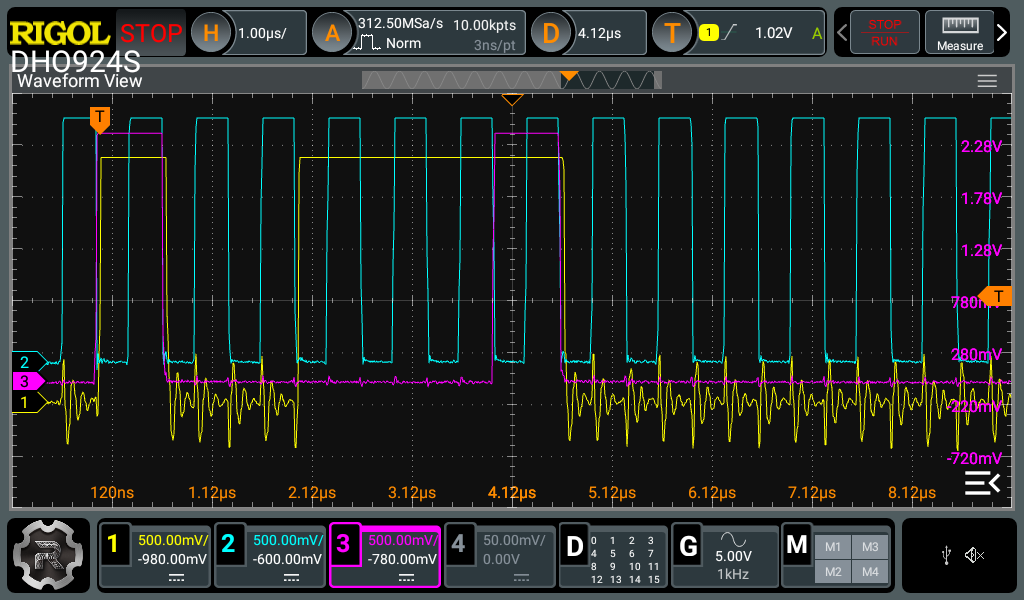
\includegraphics[width=\textwidth]{Pics/oszi_cube_spi_example.png}
	\caption{Screenshot des Osziloskopbildschirms. Dieser zeigt die Wellen für SCK (blau), MOSI (magenta) und MISO (gelb).}
	\label{fig:oszi_cube_spi_example}
\end{figure}

So sollten die Wellen auch mit dem Plattformunabhängigen Code aussehen.














































